\documentclass[12pt,a4paper]{article}
\usepackage[utf8]{inputenc}
\usepackage{amsmath}
\usepackage{listings}
\usepackage{verbatim}
\usepackage{graphicx} 
\oddsidemargin 0cm
\marginparwidth 0cm
\hoffset 0cm
\usepackage{polski}
\begin{document} 
\large
\begin{tabular}{|c|c|c|c|}
\hline
\multicolumn{4}{|l|}{Temat:}\\
\multicolumn{4}{|c|}{Interpolacja Newtona}\\
\hline
\multicolumn{1}{|l}{Wykonał:}&\multicolumn{1}{|l}{Wydział:}&\multicolumn{1}{|c}{Kierunek}&\multicolumn{1}{|l|}{Grupa:}\\
Marcin Fabrykowski&FiIS&Inf. Stos.&grupa 3\\
\hline
\end{tabular}
\normalsize
\vspace{2cm}
\begin{enumerate}
\item Wstęp\\
Aby omówić metodą interpolacji Newtona, niezbędne będzie poznanie pojęcia ilorazu różnicowego. Definiujemy go jako: $f(x_0;x_1)=\dfrac{f(x_1)-f(x_0)}{x_1-x_0}$.\\
Używając powyższego wzoru tworzymy tabelkę ilorazów. Wygląd tej tabelki pokaże w~części \textit{Wykonanie ćwiczenia}.\\
Następnie nasz szukany wielomian interpolujący wyraża się wzorem:$$W_n(x)=f(x_0)+f(x_0;x_1)\omega_0(x)+f(x_0;x_1;x_2)\omega_1(x)+\dots+f(x_0;x_1;\dots;x_n)\omega_{n-1}(x)$$
\item wykonanie ćwiczenia\\
Naszym celem będzie interpolacja funkcji $f(x)=\dfrac{1}{1+x^2}$. Zakładamy węzły interpolacji w~punktach $x_i=-5,-2,-\dfrac{1}{2},0,\dfrac{1}{2},2,5$.\\
Obliczamy wartości funkcji w~węzłach, a~następnie wykonać tabelkę ilorazów różnicowych. Mając te wartości, obliczamy wielomian interpolujący.\\
Powyższe zadania realizuje poniższy program.
\lstinputlisting[language=C++,caption=main.cpp,breakatwhitespace=true,basicstyle=\footnotesize,breaklines=true]{main.cpp}
Czego wynikiem jest poniższa tabelka ilorazów różnicowych:
\footnotesize
\verbatiminput{tabelka.dat}
\normalsize
Oraz interpolowane wartości funkcji:
\footnotesize
\verbatiminput{w.dat}
\normalsize
Co przedstawiając graficznie jako funkcję interpolowaną i~interpolującą widać na rys.
\begin{figure}
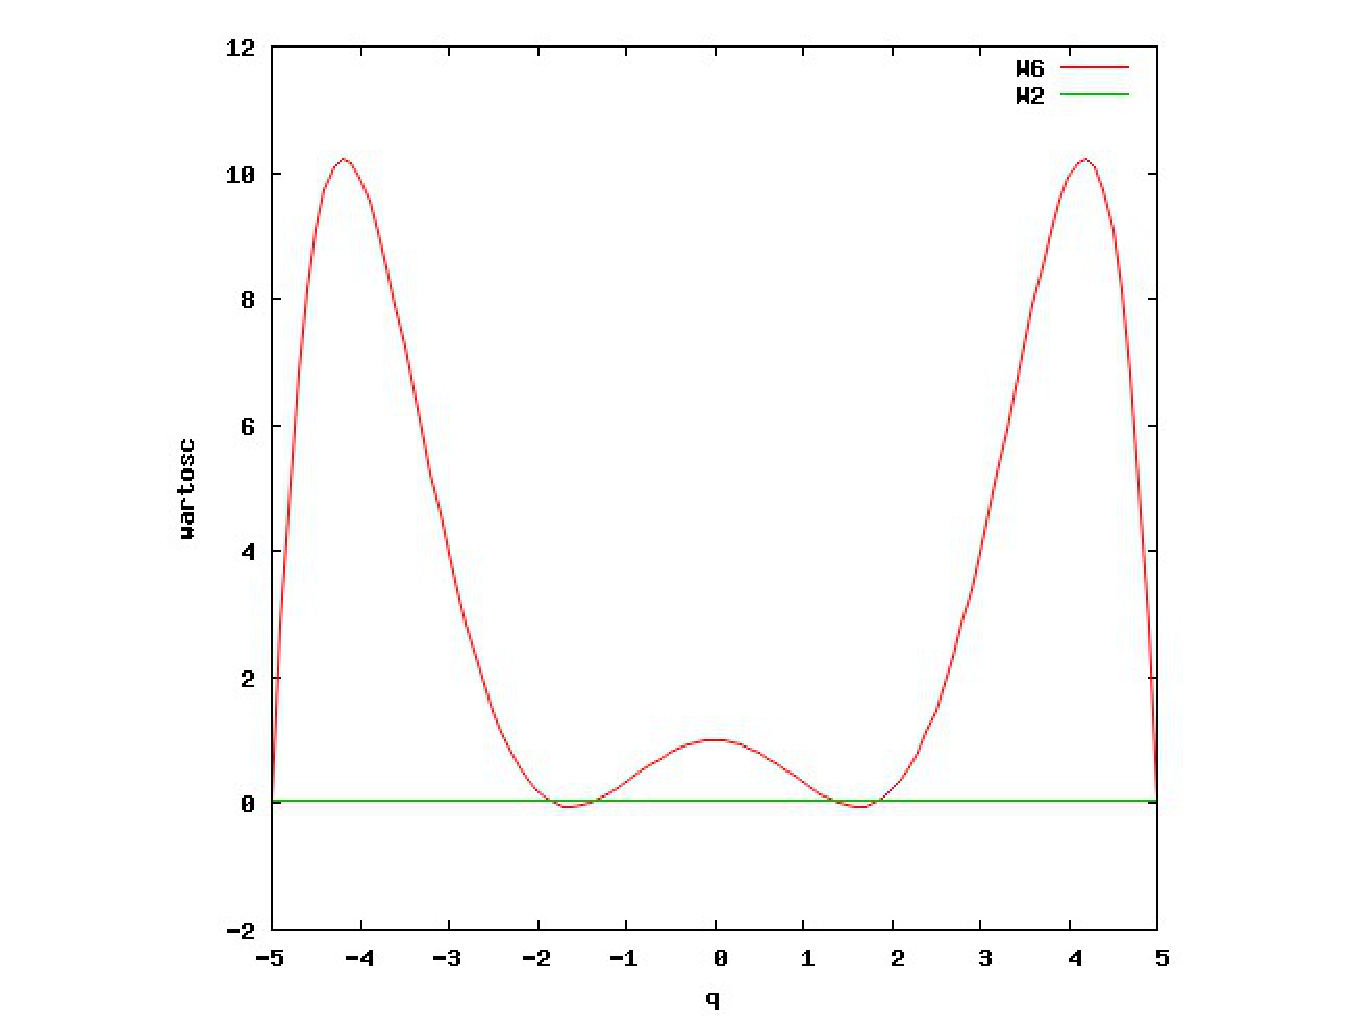
\includegraphics[scale=0.8]{plot.eps}
\end{figure}
\item Wnioski\\
Interpolacja Newtona pozwala na wyliczenie wartości funkcji w~argumentach nie będących węzłami interpolacyjnymi. Jednakże wykonanie ćwiczenia nie dało oczekiwanego wyniku interpolacyjnego, co mogło być spowodowane błędem implementacyjnym w~zastosowanym programie autorskim.
\end{enumerate}
\end{document}
